\chapter*{Experiment 4 - MP3 Player}
\addcontentsline{toc}{chapter}{Experiment 4 - MP3 Player}
We wire up the experiment as shown in the diagram fig:~\ref{fig:exp4_mp3}. And upload the sketch code in the next section on page:~\pageref{sketch:exp4}.

%
\begin{figure}[ht]
	\centering
	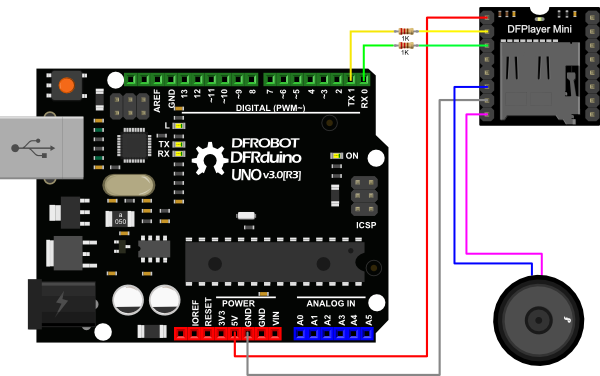
\includegraphics[width=12cm]{images/11}
	\caption{Read a buttons input \citep{dfrobot-15a}}
	\label{fig:exp4_mp3}
\end{figure}
%

This example requires that a library be loaded in order to use, a copy of which is available in the companion code associated with this workshop, see also:~\citep{dfrobot-15b}. Instructions for installing a library can be found at the following url: https://www.arduino.cc/en/Guide/Libraries\#.UxU8mdzF9H0 

\newpage
\section*{Sketch Code}
\label{sketch:exp4}
\begin{lstlisting}
/*
Sample code to work with the DFPlayer Mini MP3 Player

Author: David Kirwan
Licence: Apache 2.0
*/
// libraries
#include <SoftwareSerial.h>
#include <DFPlayer_Mini_Mp3.h>

boolean playing; // Create a variable called playing

void setup () {
  Serial.begin (9600);
  mp3_set_serial (Serial);
  delay(1);
  mp3_set_volume (7);
  playing = false;
}

void loop () {
  if(!playing){
    playing = true;
    mp3_play ();
  }
}

/*
  mp3_play (); //start play
  mp3_play (5); //play "mp3/0005.mp3"
  mp3_next (); //play next
  mp3_prev (); //play previous
  mp3_set_volume (uint16_t volume); //0~30
  mp3_set_EQ (); //0~5
  mp3_pause ();
  mp3_stop ();
  void mp3_get_state ();
  void mp3_get_volume ();
  void mp3_get_u_sum ();
  void mp3_get_tf_sum ();
  void mp3_get_flash_sum ();
  void mp3_get_tf_current ();
  void mp3_get_u_current ();
  void mp3_get_flash_current ();
  void mp3_single_loop (boolean state);
  void mp3_DAC (boolean state);
  void mp3_random_play ();
*/

\end{lstlisting}